\documentclass[main.tex]{subfiles} % Subfile-Class


% ============================================================================== %
%                            Subfile document                                    %
% ============================================================================== %

\begin{document}

% Template

\subsubsection{Sensorik Strecken Rückverfolgung}

Der Algorithmus setzt voraus, dass das Gerät immer und zu jeder Zeit seine
Orientierung als absoluten Winkel ab dem Startpunkt weiss und die zurückgelegte
Strecke messen kann. Dieser Abschnitt behandelt, wie der Pfadfinder eben diese
Information erfasst. Abbildung~\ref{fig:Blockschaltbild_StreckenTracken} zeigt
schematisch auf, wie diese Funktion umgesetzt wird. Die danach folgende
Beschreibung führt dieses Schema nochmal aus.

\begin{figure}[H]
    \centering
    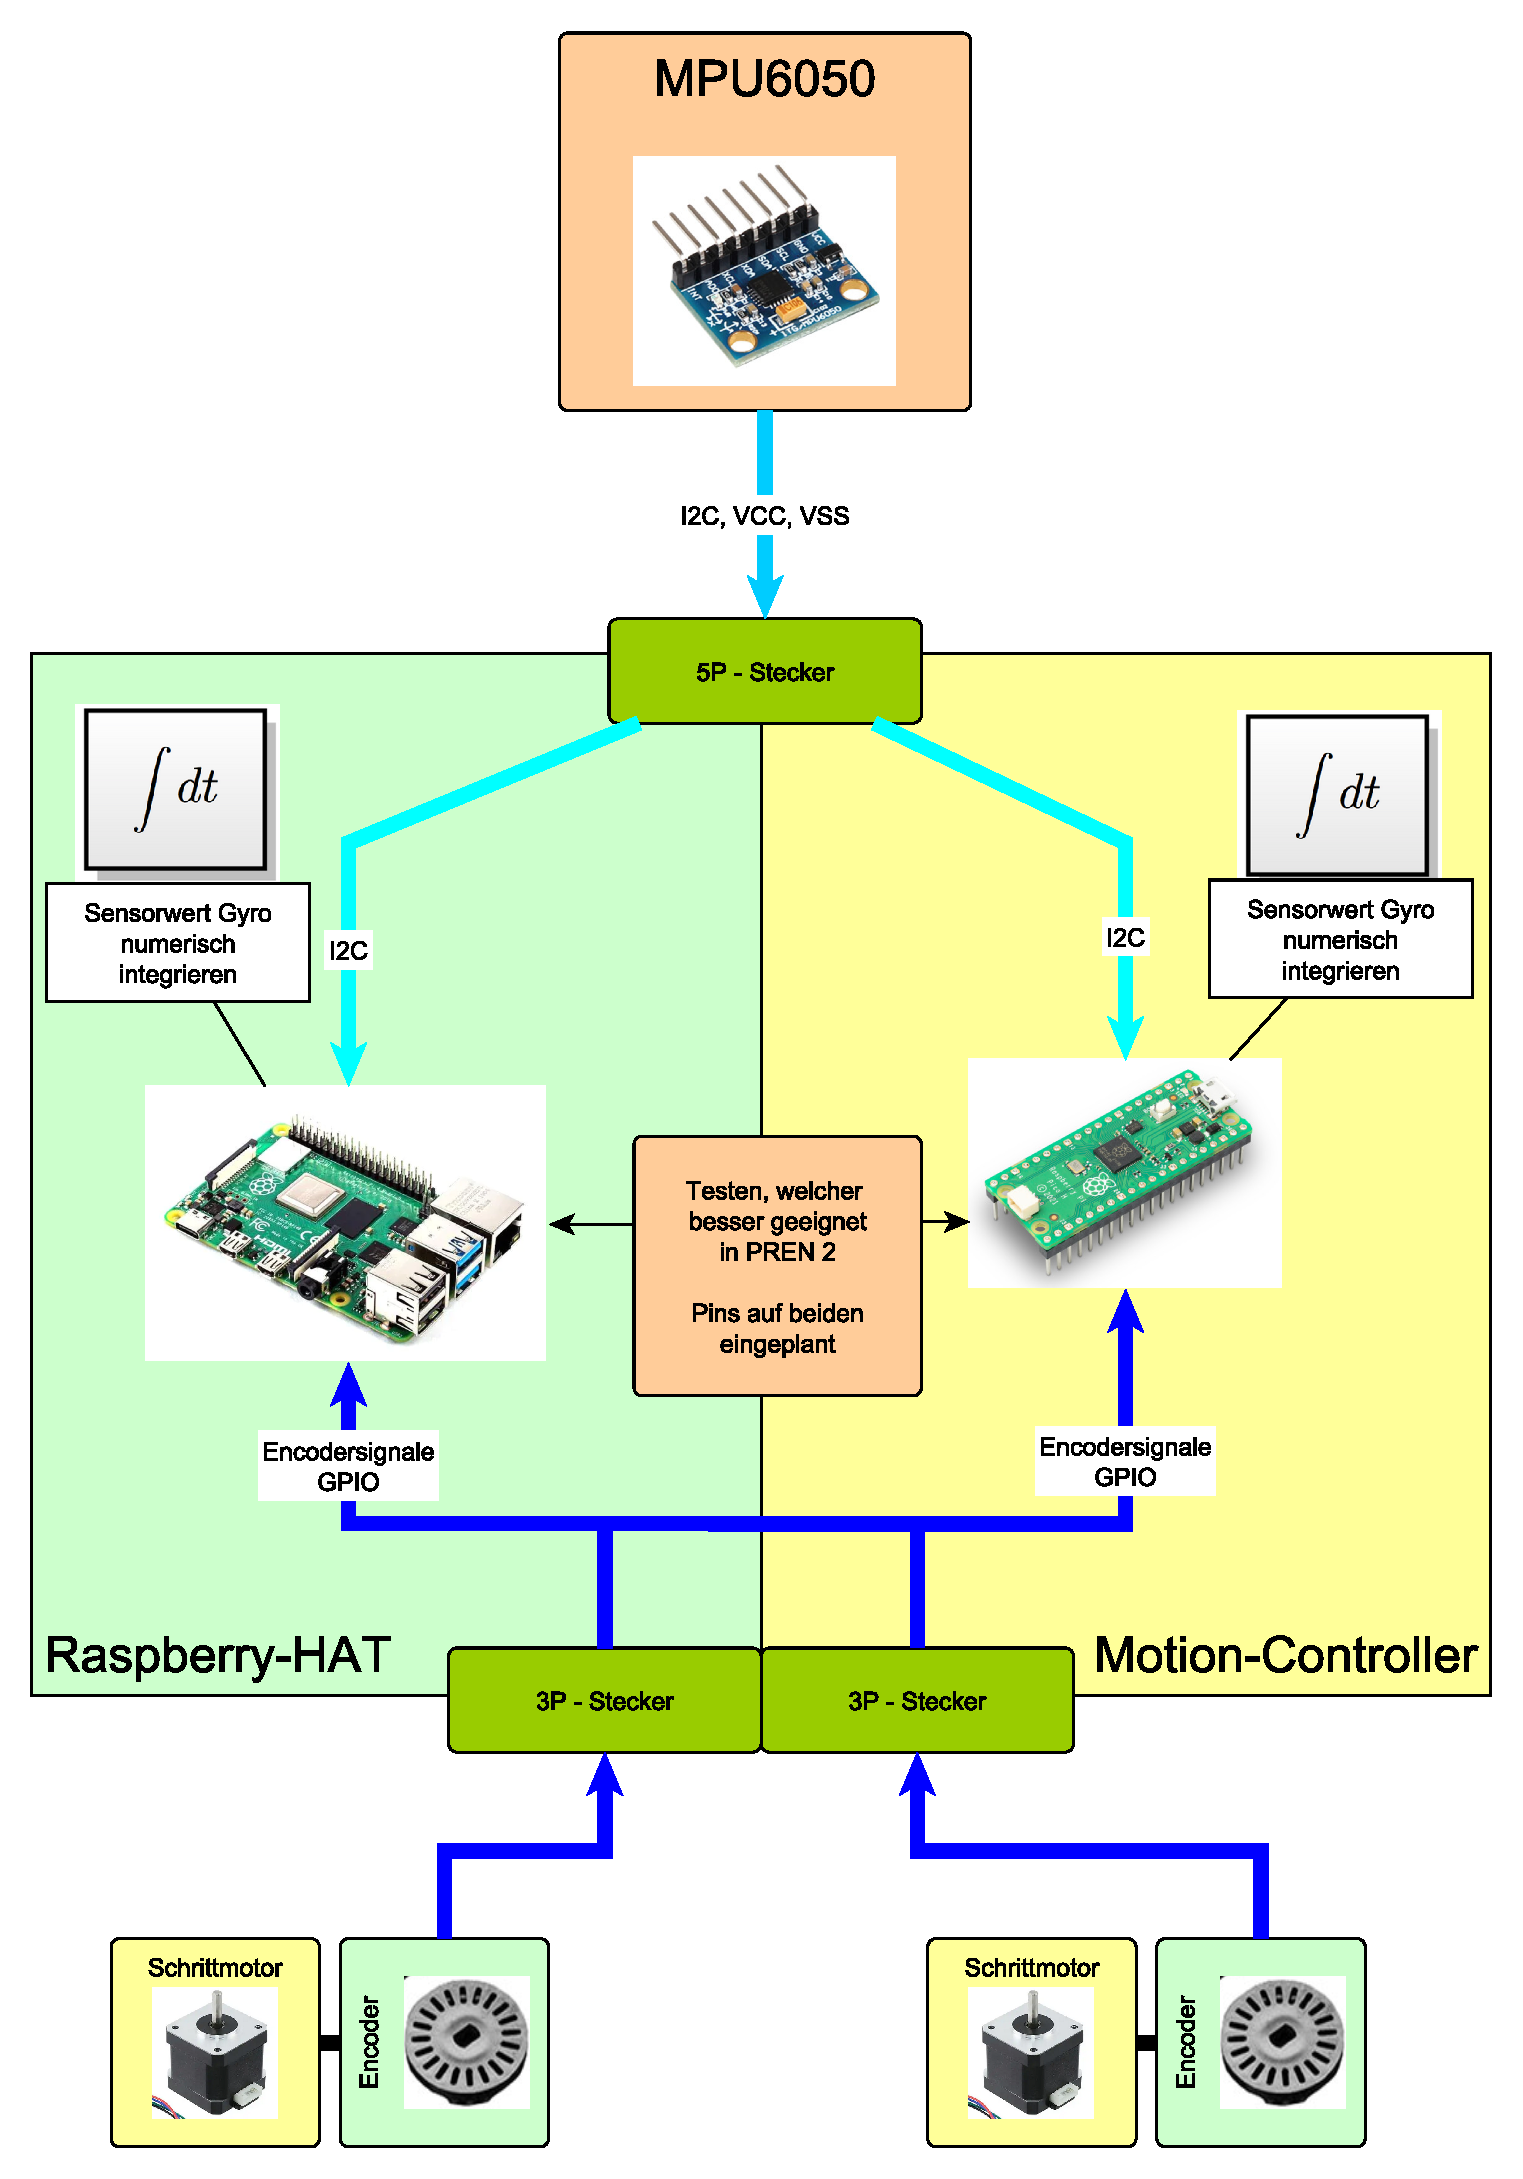
\includegraphics[width=0.75\textwidth]{./fig_Strecke_Tracken/Topologie_MPU6050.pdf}
    \caption{Blockschaltbild Sensorik Streckenrückverfolgung}~\label{fig:Blockschaltbild_StreckenTracken}
\end{figure}

% ===================================================================================
\paragraph{Winkelerfassung}
Der Winkel des Pfadfinders wird, wie in Anhang~\ref{appendix:Strecke_Tracken}
konzeptioniert, über ein Gyroskop ermittelt. Dieses erfasst die Änderungsrate
des aktuellen Winkels zu jeder Zeit und integriert sie jede $25\mu s$ numerisch
auf. Dadurch kann eine sehr genaue Angabe darüber getroffen werden, in welcher
Orientierung sich das Gerät aktuell befindet.

Mangels Echtzeitfähigkeit ist es nicht sicher, ob der Raspberry Pi in der Lage
ist, das Gyroskop ausreichend genau und häufig auszulesen. Deshalb wird ein
entsprechender Steckplatz sowohl auf dem Antriebs-Controller, als auch auf dem
Raspberry-HAT vorgesehen, um dies im Nachfolgemodul PREN2 noch zu testen.

\paragraph{Zurückgelegte Strecke}
Wie in der Konzeption beschrieben, wird die zurückgelegte Strecke des 
Pfadfinders mithilfe eines Encoders erfasst. Die verwendete Lochscheibe 
besitzt 36 Löcher, was einer Auflösung von 10 Grad pro Schritt entspricht. 
Die Dimensionen der Löcher wurden basierend auf den Herstellerangaben aus 
dem entsprechenden Datenblatt festgelegt. Laut Hersteller beträgt die 
minimale Erfassungsgrösse 1.8 x 0.8 mm, weshalb Löcher mit den Abmessungen 
1.8 x 1.6 mm gewählt wurden 
(siehe Abbildung~\ref{fig:Lochscheibe_Vermasst}).

Falls sich während der Tests in PREN 2 herausstellt, dass die Auflösung nicht 
ausreicht, könnte der Durchmesser der Lochscheibe vergrössert werden, um bei 
gleichbleibender Lochgrösse mehr Löcher pro Umdrehung unterzubringen.

\begin{figure}[H]
    \centering
    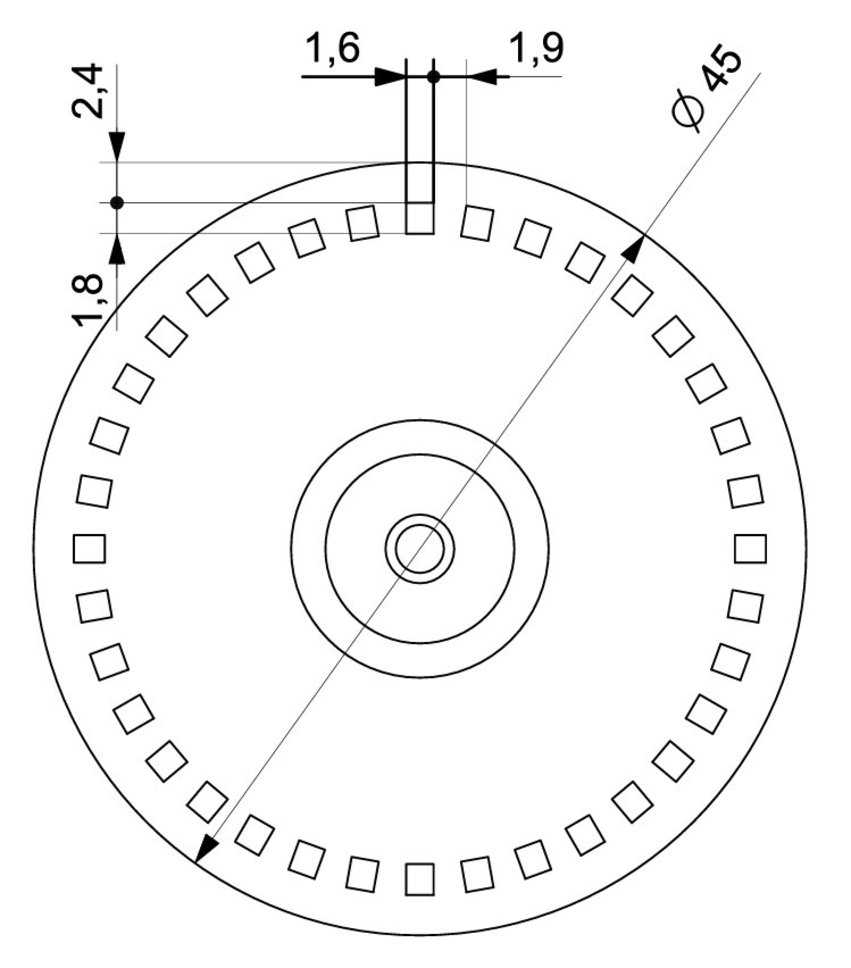
\includegraphics[width=0.5\textwidth]{./fig_Strecke_Tracken/Encoderscheibe_Vermasst.pdf}
    \caption{Masse der Lochscheibe}~\label{fig:Lochscheibe_Vermasst}
\end{figure}

In einem zweiten Versuch soll im Folgemodul PREN2 getestet werden, ob es
ausreichen könnte, die zurückgelegten Schritte des Schrittmotorentreibers für
diese Referenz zu verwenden. Dieser Versuch kann allerdings erst ausreichend
aussagekräftig durchgeführt werden, wenn ein erster Roboter gebaut ist.

\end{document}